\documentclass{beamer}

\usepackage{amsmath}
\usepackage{graphicx}
\usepackage{amssymb}

\begin{document}
\section*{Part 3 Anonymisation Methods}	
	
%=========================================================%
%% 3.2  Local Suppression
%% 3.3. Post-randomization (PRAM)

%% 3.4  MicroAggregation
%% 3.5  Adding Noise
%% 3.6  Shuffling
 
 
% % Section  4 MEASURING DATA UTILITY AND INFORMATION LOSS

\begin{frame}

\frametitle{ Anonymisation Methods}
\begin{itemize}
\item Two kinds of anonymization methods:
\item[1.] deterministic 
\item[2.] probabilistic. 
\bigskip
\item \textbf{Categorical Variables:}\\ For categorical variables, recoding and local suppression are deterministic
procedures (they are not influenced by randomness), while swapping and PRAM are based on randomness and considered probabilistic
methods. 
% [\textit{Gouweleeuw ct al., 1998}] 
\end{itemize}
\end{frame}
\begin{frame}
	
	\frametitle{ Anonymisation Methods}
	\begin{itemize}
\item 
For continuous variables, \textbf{micro-aggregation} is a deterministic method,
while\textbf{ adding correlated noise}  and \textbf{shuffling}
are probabilistic procedures. 
\bigskip
% -  [\textit{Muralidhar et al., 1999}]
\item \textbf{Reproducibility}: Whenever probabilistic methods are applied, the random seed of the software’s pseudo random number generator should be fixed to
ensure reproducibility of the results.
\end{itemize}
\end{frame}
%======================================================================= %
\begin{frame}
	\Large
Anonymisation Methods
\begin{enumerate}	
	\item Recoding
	\item Local Suppression
	\item Post-randomization (PRAM)
	\item Micro-aggregation
	\item Adding Noise
	\item Shuffling
\end{enumerate}
\end{frame}
%===============================================%
\begin{frame}
\frametitle{1. Recoding}
\begin{itemize}
\item Global recoding is a non-perturbative method that can be applied to both categorical and continuous key variables.
\item \textbf{Fundamental Idea:} The basic idea of recoding a categorical variable
is to combine several categories into a new, less informative category. 
\item \textbf{Examples} A frequent
use case is the recoding of age given in years into age groups.
\item  If the method is applied to a continuous variable, it means to discretize the variable. 
\item An application
would be the to split a variable containing incomes some income groups.
\item Remark: Bins for Histograms
%% Page 14 / 31
%% 3 AN ON YMISATI ON METHODS
\end{itemize}
\end{frame}


%==================================================== %
\begin{frame}
	\frametitle{1. Recoding}
	\begin{itemize}
\item The goal in both cases is to reduce the total number of possible outcomes of a
variable. 
\item Typically, recoding is applied to categorical variables where the number
of categories with only few observations (i.e., extreme categories such as persons
being older than 100 years) is reduced. 
\item A typical example would be to combine
certain economic branches or to build age classes from the variable age.
\end{itemize}
\end{frame}
%==================================================== %
\begin{frame}
	\frametitle{1. Recoding}
	\begin{itemize}
\item A special case of global recoding is \textbf{top and bottom coding}, which can be applied
to ordinal and categorical variables. 
\item The idea for this approach is that all values
above (i.e., top coding) and / or below (i.e., bottom coding) a pre-specified threshold
value are combined into a new category. 
\item \textbf{Examples} Heights and Weights
\end{itemize}
\end{frame}
%==================================================== %
\begin{frame}
	\frametitle{1. Recoding}
\textbf{Implementation}
	\begin{itemize}
%\item A typical use case for top-coding is to recode all values of a variable containing age in years that are above 80 into a new category 80+.

%--------------------------------------------------------------------%
\item Function \texttt{globalRecode()} can be applied in \textbf{sdcMicro} to perform both global
recoding and top/bottom coding. 
\item The \textbf{sdcMicroGUI} offers a more user-friendly
way of applying global recoding.
\end{itemize}
\end{frame}

%==================================================== %
\begin{frame}
	\frametitle{2. Local Suppression}
	\begin{itemize}
\item Local suppression is a non-perturbative method that is typically applied to categorical variables to suppress certain values in at least one variable. 
\item Normally, the
input variables are part of the set of key variables that is also used for calculation
of individual risks. %, as described in Section 2. 

\item Individual values are suppressed
in a way that the set of variables with a specific pattern are increased.
\item Local
suppression is often used to achieve \textbf{k-Anonymity}. %, as described in Section 2.2.
\end{itemize}
\end{frame}
%==================================================== %
\begin{frame}
	\frametitle{2. Local Suppression}
\textbf{Implementation}
	\begin{itemize}
		\item Using function \texttt{localSupp()} of \textbf{sdcMicro}, it is possible to suppress the values of
a key variable for all units having individual risks above a pre—defined threshold,
given a disclosure scenario. 


\item This procedure requires user intervention by setting
the threshold. 
\item To automatically suppress a minimum amount of values in the key
variables to achieve k-anonymity, one can use function \texttt{localSuppression()}.
\item This
algorithm also allows specification of a user-dependent reference that determines
which key variables are preferred when choosing values that need to be suppressed.
\end{itemize}
\end{frame}
%==================================================== %
\begin{frame}
	\frametitle{2. Local Suppression}
	\begin{itemize}
\item ln this implementation, a heuristic algorithm is called to suppress as few values
as possible. It is possible to specify a desired ordering of key variables in terms of
importance, which the algorithm takes into account. 
\item lt is even possible to specify
key variables that are considered of such importance that almost no values for
these variables are suppressed.
\item This function can also be used in the graphical
user interface of the \textbf{sdcMicroGUI} package.
\end{itemize}
\end{frame}
%==================================================== %
\begin{frame}
	\frametitle{3. Post-randomization (PRAM)}
\begin{itemize}

\item \textbf{Post-randomization} - PRAM is a perturbation, probabilistic method that can be applied to categorical variables. 

\item The idea is that the values of a categorical variable in the original microdata file are changed into other categories, taking into account pre-defined transition probabilities.
\item This process is
usually modeled using a \textbf{known transition matrix}. 

\item For each category of a categorical variable, this matrix lists probabilities to change into other possible categories.
\end{itemize}
\end{frame}
%==================================================== %
\begin{frame}
	\frametitle{3. Post-randomization (PRAM)}
\textbf{Examples}\\
	\begin{itemize}


\item 

As an example, consider a variable with only 3 categories: Al, A2 and A3. 
\item The
transition of a value from category A1 to category A1 is, for example, fixed with
probability $P_1 = 0.85$, which means that only with probability $p_1 = 0.15$ can a
value of A1 be changed to either A2 or A3. 
\item The probability of a change from category A1 to A2 might be fixed with probability $P_2 = 0.1$ and changes from A1
to A3 with $p_3 = 0.05$. 
%% Page 15 / 31
%% 3 AN ON YMISATI ON METHODS

\end{itemize}
\end{frame}
%==================================================== %
\begin{frame}
	\frametitle{3. Post-randomization (PRAM)}
	\textbf{Examples}\\
	\begin{itemize}

\item Probabilities to change values from class A2 to other classes
and for A3, respectively, must be specified beforehand. 
\item All transition probabilities
must be stored in a matrix that is the main input to function \texttt{pram()} in sdcMicro.

\item PRAM is applied to each observation independently and randomly.
\item This means
that different solutions are obtained for every run of PRAM if no seed is specified
for the random number generator. 
\item A main advantage of the PRAM procedure is
the flexibility of the method. 
\end{itemize}
\end{frame}

%==================================================== %
\begin{frame}
	\frametitle{3. Post-randomization (PRAM)}
	\textbf{Examples}\\
	\begin{itemize}
\item Since the transition matrix can be specified freely as a
function parameter, all desired effects can be modeled. 
\item For example, it is possible
to prohibit changes from one category to another by setting the corresponding
probability in the transition matrix to 0.

\item In \textbf{sdcMicro} and \textbf{sdcMicroGUI}, \texttt{pram\_strat()} allows PRAM to be performed.
%The corresponding help file can be accessed by typing ?pram into an R console or using the help-menu of sdcMicroGUI. 
\end{itemize}
\end{frame}
%==================================================== %
\begin{frame}
	\frametitle{3. Post-randomization (PRAM)}
	\textbf{Examples}
	\begin{itemize}
\item When using \texttt{pram\_strat()}, it is possible
to apply PRAM to sub-groups of the micro dataset independently. \item In this case,
the user needs to select the stratification variable defining the sub-groups. \item If
the specification of this variable is omitted, the PRAM procedure is applied to
all observations in the dataset.
\end{itemize}
\end{frame}
%==================================================== %
\begin{frame}
	\frametitle{3. Post-randomization (PRAM)}
	\textbf{Examples}
	\begin{itemize} \item  We note that the output of PRAM is slightly
different in \textbf{sdcMicroGUI}. 
\item In this case for each variable values \texttt{nrChanges} shows
the total number of changed values for a given variable while \texttt{percChanges} lists the
percentage of changed values any variable for which PRAM has been applied.
\end{itemize}
\end{frame}

%==================================================== %
\begin{frame}
	\frametitle{4. Microaggregation}
	\textbf{Examples}\\
	\begin{itemize}

\item Micro-aggregation is a perturbative method that is typically applied to continuous
variables. The idea is that records are partitioned into groups; within each group,
the values of each variable are aggregated. 
\item Typically, the arithmetic mean is used
to aggregate the values, but other robust methods are also possible. 
\item Individual
values of the records for each variable are replaced by the group aggregation value,
which is often the mean; as an example, see Table 4, where two values that are
most similar are replaced by their column-wise means.

\end{itemize}
\end{frame}
%================================================================55
\begin{frame}
\begin{figure}
\centering
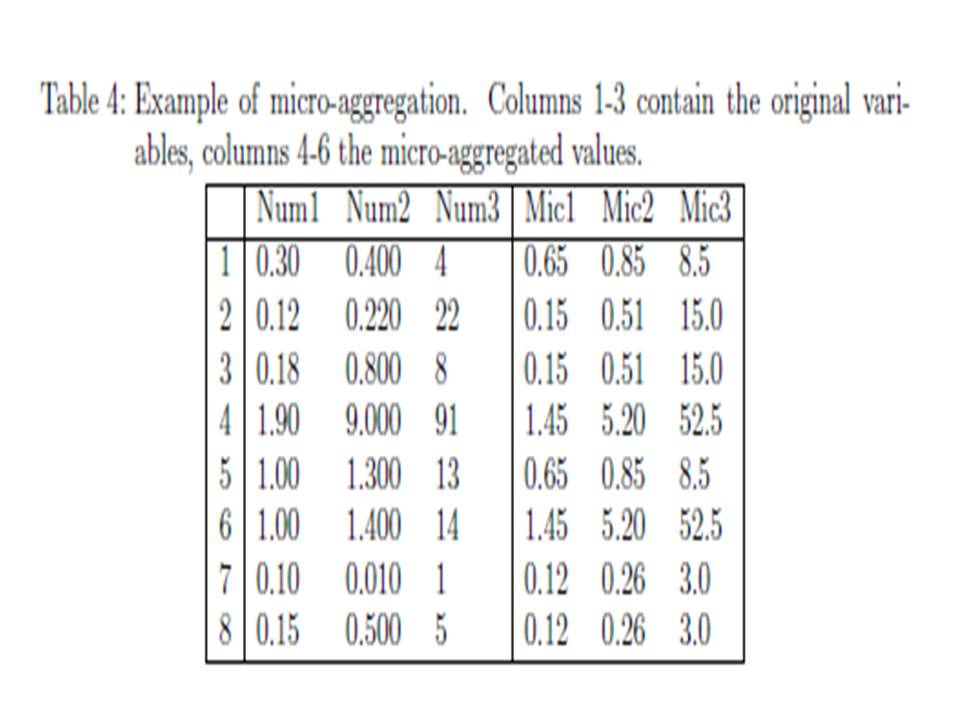
\includegraphics[width=0.89\linewidth]{TemplJPGs2/Slide3}
\end{figure}

\end{frame}
%==================================================== %
\begin{frame}
	\frametitle{4. Microaggregation}
\textbf{Implementation}
	\begin{itemize}
		
% % Table 4
\item Depending on the method chosen in function \texttt{microaggregation()}, additional
parameters can be specified. 
\item For example, it is possible to specify the number of
observations that should be aggregated as well as the statistic used to calculate
the aggregation. 
\item It is also possible to perform micro—aggregation independently to
pre-defined clusters or to use cluster methods to achieve the grouping.

\end{itemize}
\end{frame}
%==================================================== %
%\begin{frame}
%	\frametitle{4. Microaggregation}
%	\textbf{Examples}\\
%
%%% Page 16 / 31
%%% 3 AN ON YMISATI ON METHODS
%However, computationally it is the most challenging task to find a good partition
%of the observations to groups. 
%
%\end{frame}
%==================================================== %
\begin{frame}
\frametitle{Methods for Micro-Aggregation}
In \textbf{sdcMicroGUI}, several different methods for micro-aggregation are available
\begin{itemize}
\item \texttt{mdav}: grouping is based on classical (Euclidean) distance measures.
\item \texttt{rmd}: grouping is based on robust multivariate (Mahalanobis) distance measures.
\item \texttt{pca}: grouping is based on principal component analysis whereas the data
are sorted on the first principal component.
\item \texttt{clustpppca}: grouping is based on clustering and (robust) principal component analysis for each cluster.


\item \texttt{Influence}: grouping is based on clustering and aggregation is performed within clusters.
\end{itemize}
\end{frame}
%==================================================== %
\begin{frame}
	\begin{itemize}
\item For computational reasons it is recommended to use the highly efficient implementation of method \texttt{mdav}. 
\item It is almost as fast as the \texttt{pca} method, but performs
better. 
\item For data of moderate or small size, method \texttt{rmd} is favorable since the
grouping is based on multivariate (robust) distances.

\item All of the previous settings (and many more) can be applied in \textbf{sdcMicro}, using
function \texttt{microaggregation()}.
\end{itemize} 
\end{frame}
\end{document}
% The corresponding help file can be viewed with command \texttt{?microaggregation} or by using the help-menu in sdcMicroGUI.
\newpage